\documentclass[../main.tex]{subfiles}
\graphicspath{{\subfix{../../images/}}}
\begin{document}


\chapter{Task Performance}\label{chap:performance}


\begin{quote}
    \emph{Perception is not something that happens to us, or in us, \lbrack\ldots\rbrack It is something we do.}\\ 
    \raggedleft{--- Alva Noë, Perception in Action}
\end{quote}

\begin{quote}
    \emph{Because some tasks require that certain components be mastered before other components can be performed or even attempted, there is likely to be a typical developmental sequence in acquiring certain skills. Furthermore, if substantial work is required for component processes to reach a level of mastery before higher level tasks can be attempted, then there is likely to be some period of consolidation in the acquisition of the higher level skill. That is, there will be periods in which there appears to be little progress being made in performance of the task. Closer scrutiny, however, may reveal that performance is improving, but only on lower level components of the task. According to this view of skill acquisition, then, the processes that underlie plateaus in learning curves may also underlie the stages that are characteristic of cognitive development}\\
    \raggedleft{--- Piaget, 1953}
\end{quote}

\begin{quote}
    \emph{The motor learning field does not yet possess an adequate computational model for practice-induced increases in motor acuity.}\\
    \raggedleft{--- Krakauer et al. 2019}
\end{quote}

\begin{quote}
    \emph{An interesting open question is how to relate trial-to-trial dynamics of learning to asymptotic predictions regarding optimal adaptation.}\\
    \raggedleft{--- Todorov, 2007}
\end{quote}

\cleardoublepage%


\section{Does Subject Performance Improve over Trials?}

Are subjects actually learning the task? 
    Hypothesis: Yes! Across various measures of performance, the majority of subjects learn to achieve the task’s goals in the allotted time period.

Is the task difficult enough to pose a learning challenge for subjects?
    Hypothesis: yes, some subjects struggle to learn the task, some subjects learn very quickly, while the majority of subjects are between these two extremes. Learning curves are “stretched” across the allotted learning period.


Is there variability across subjects in terms of performance?
    Hypothesis --- yes! And now we want to understand what correlates with particular subject performance


we see an interaction between learning systems -- cortex, cerebellum, basal ganglia -- strategy / unsupervised prediction / supervised, RL / policies? this leads to multiple learning rates, fast and slow learning, discontinuities in learning

skill learning will lead to hierarchy, and different levels of the hierarchy may be learned at different times by different means/systems

what do our learning curves look like? plateaus? discontinuities?

what you're learning is dimensions of goal-relevance. as these dimensions are learned, we see changes in variability and in performance


\begin{figure}[tph]
    \centering
    \includegraphics[width=1.0\textwidth]{basic_results/performance_over_blocks/hits_and_noholds.pdf}
    \caption[Hit counts over trials]{Task outcomes over blocks. Outcomes across all 45 blocks of 12 trials (targets) in the ``center hold, reach out'' task. Subjects with the most, median, and least hits are shown in green, blue, and orange respectively. All ofther subjects are show in gray. From top to bottom: The percentage of ``Hits'' within each block, the percentage of ``Misses'' (timeouts), and ``No Holds'' (subject unable to quiet forearm muscle activity initially).}\label{fig:hits_and_noholds}
\end{figure}


\begin{figure}[tph]
    \centering
    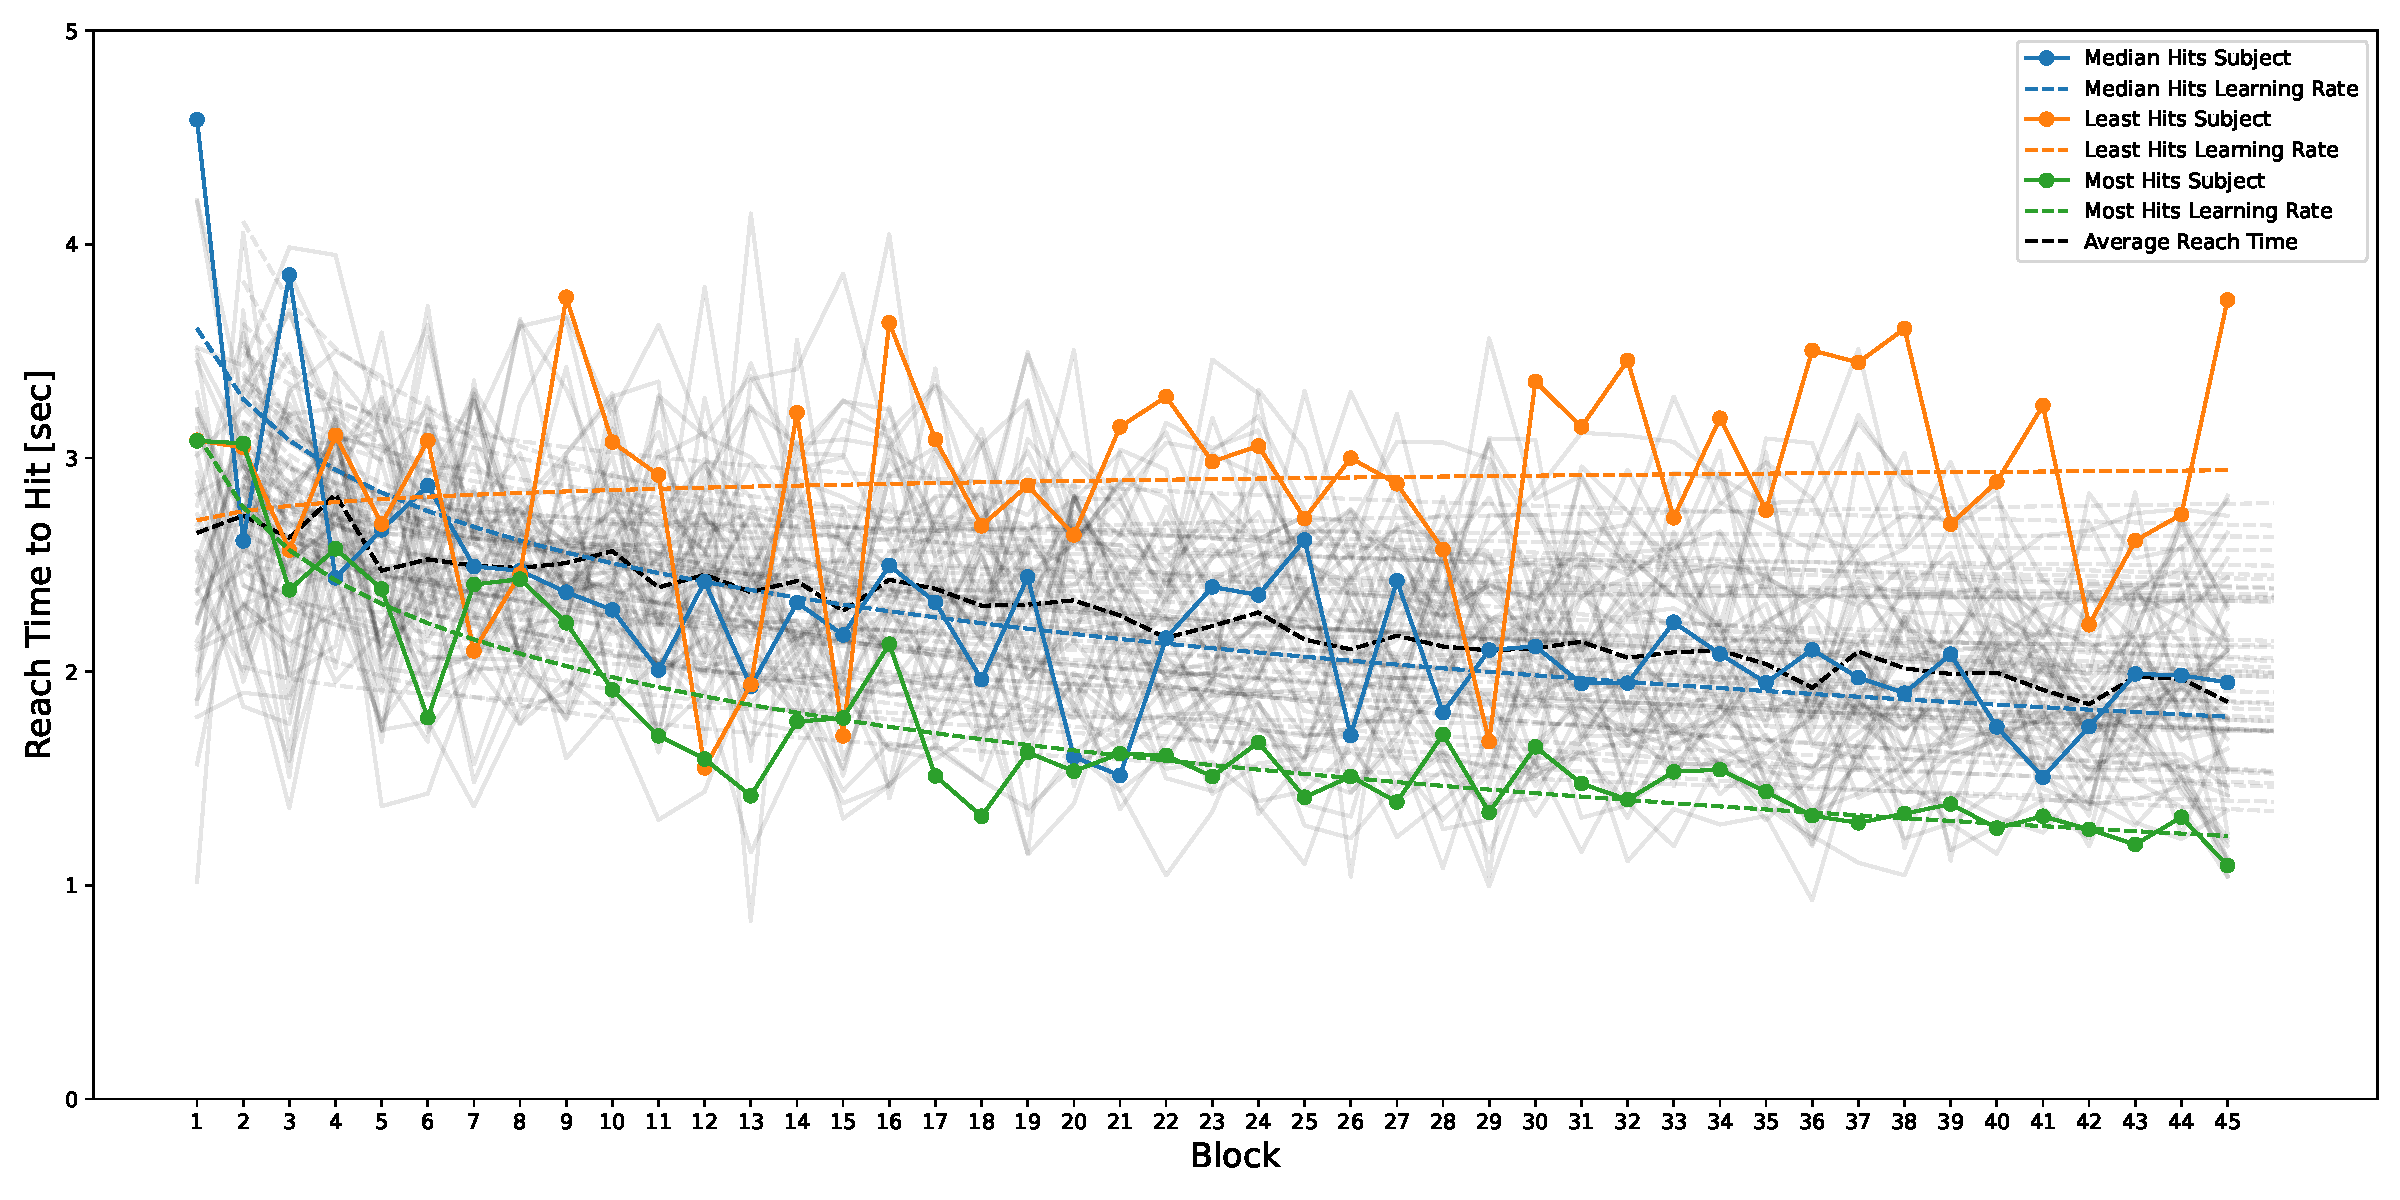
\includegraphics[width=1.0\textwidth]{basic_results/performance_over_blocks/reach_times_over_blocks.pdf}
    \caption[Reach time over trials]{}\label{fig:reach_times_over_blocks}
\end{figure}


\begin{figure}[tph]
    \centering
    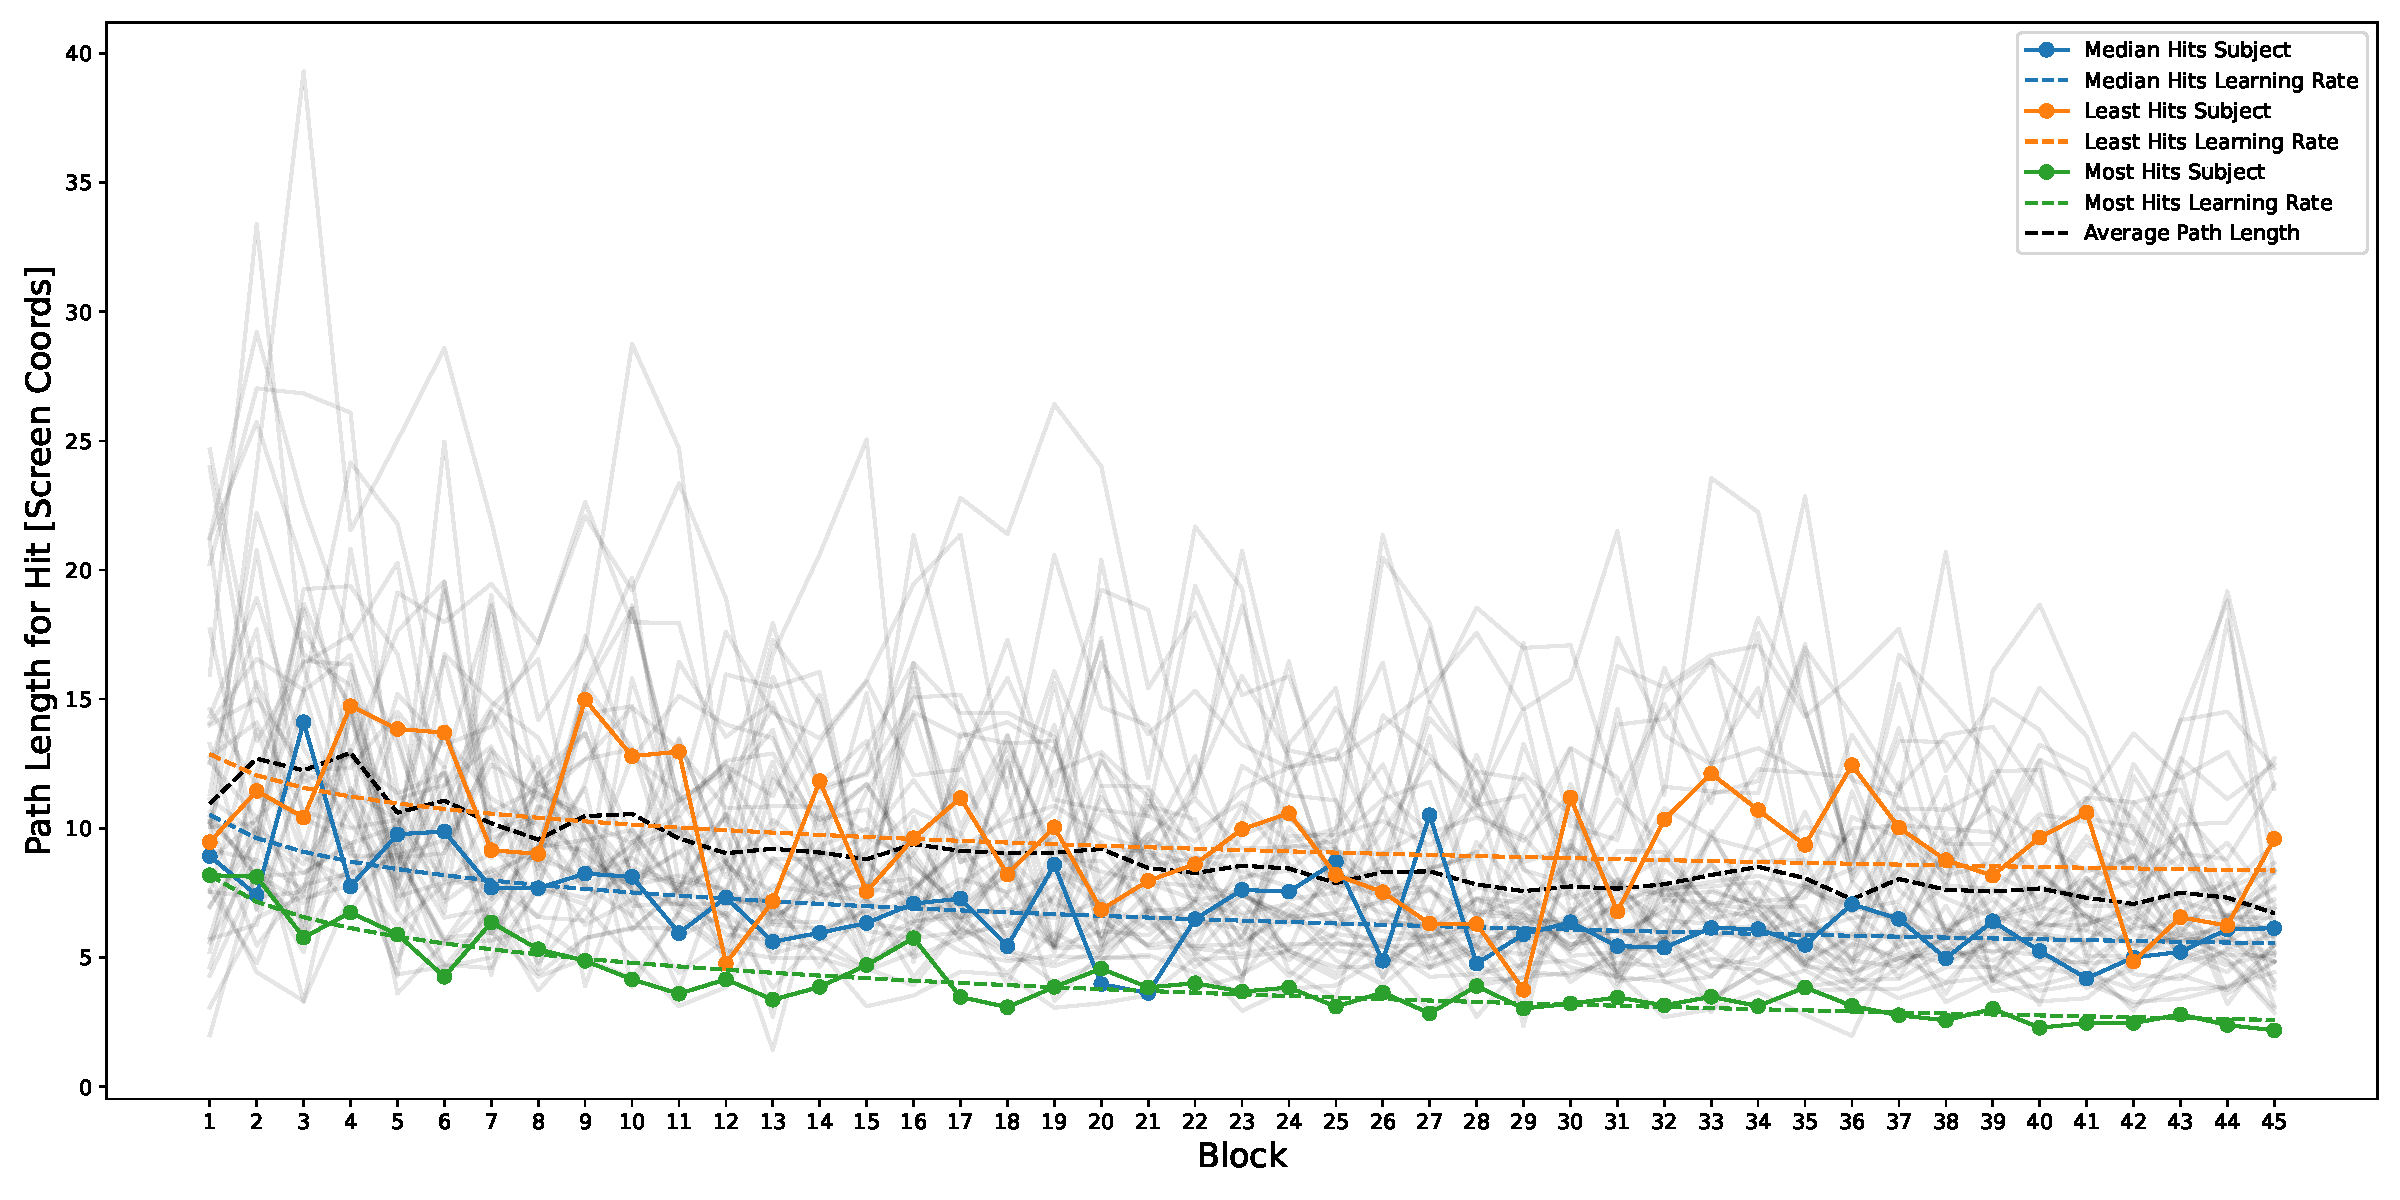
\includegraphics[width=1.0\textwidth]{basic_results/performance_over_blocks/path_length_over_blocks.pdf}
    \caption[Trajectory length over trials]{return np.sum (np.sqrt (np.sum (np.diff (a, axis=0)**2,axis=1)))}\label{fig:path_length_over_blocks}
\end{figure}


\begin{figure}[tph]
    \centering
    \includegraphics[width=1.0\textwidth]{basic_results/performance_over_blocks/path_segments_over_blocks.pdf}
    \caption[Trajectory segments over trials]{This connects to the idea of freezing degrees of freedom. We expect to see degrees of freedom in the task space, quantified by segments, to decrease over trials.}\label{fig:path_segments_over_blocks}
\end{figure}


\begin{figure}[tph]
    \centering
    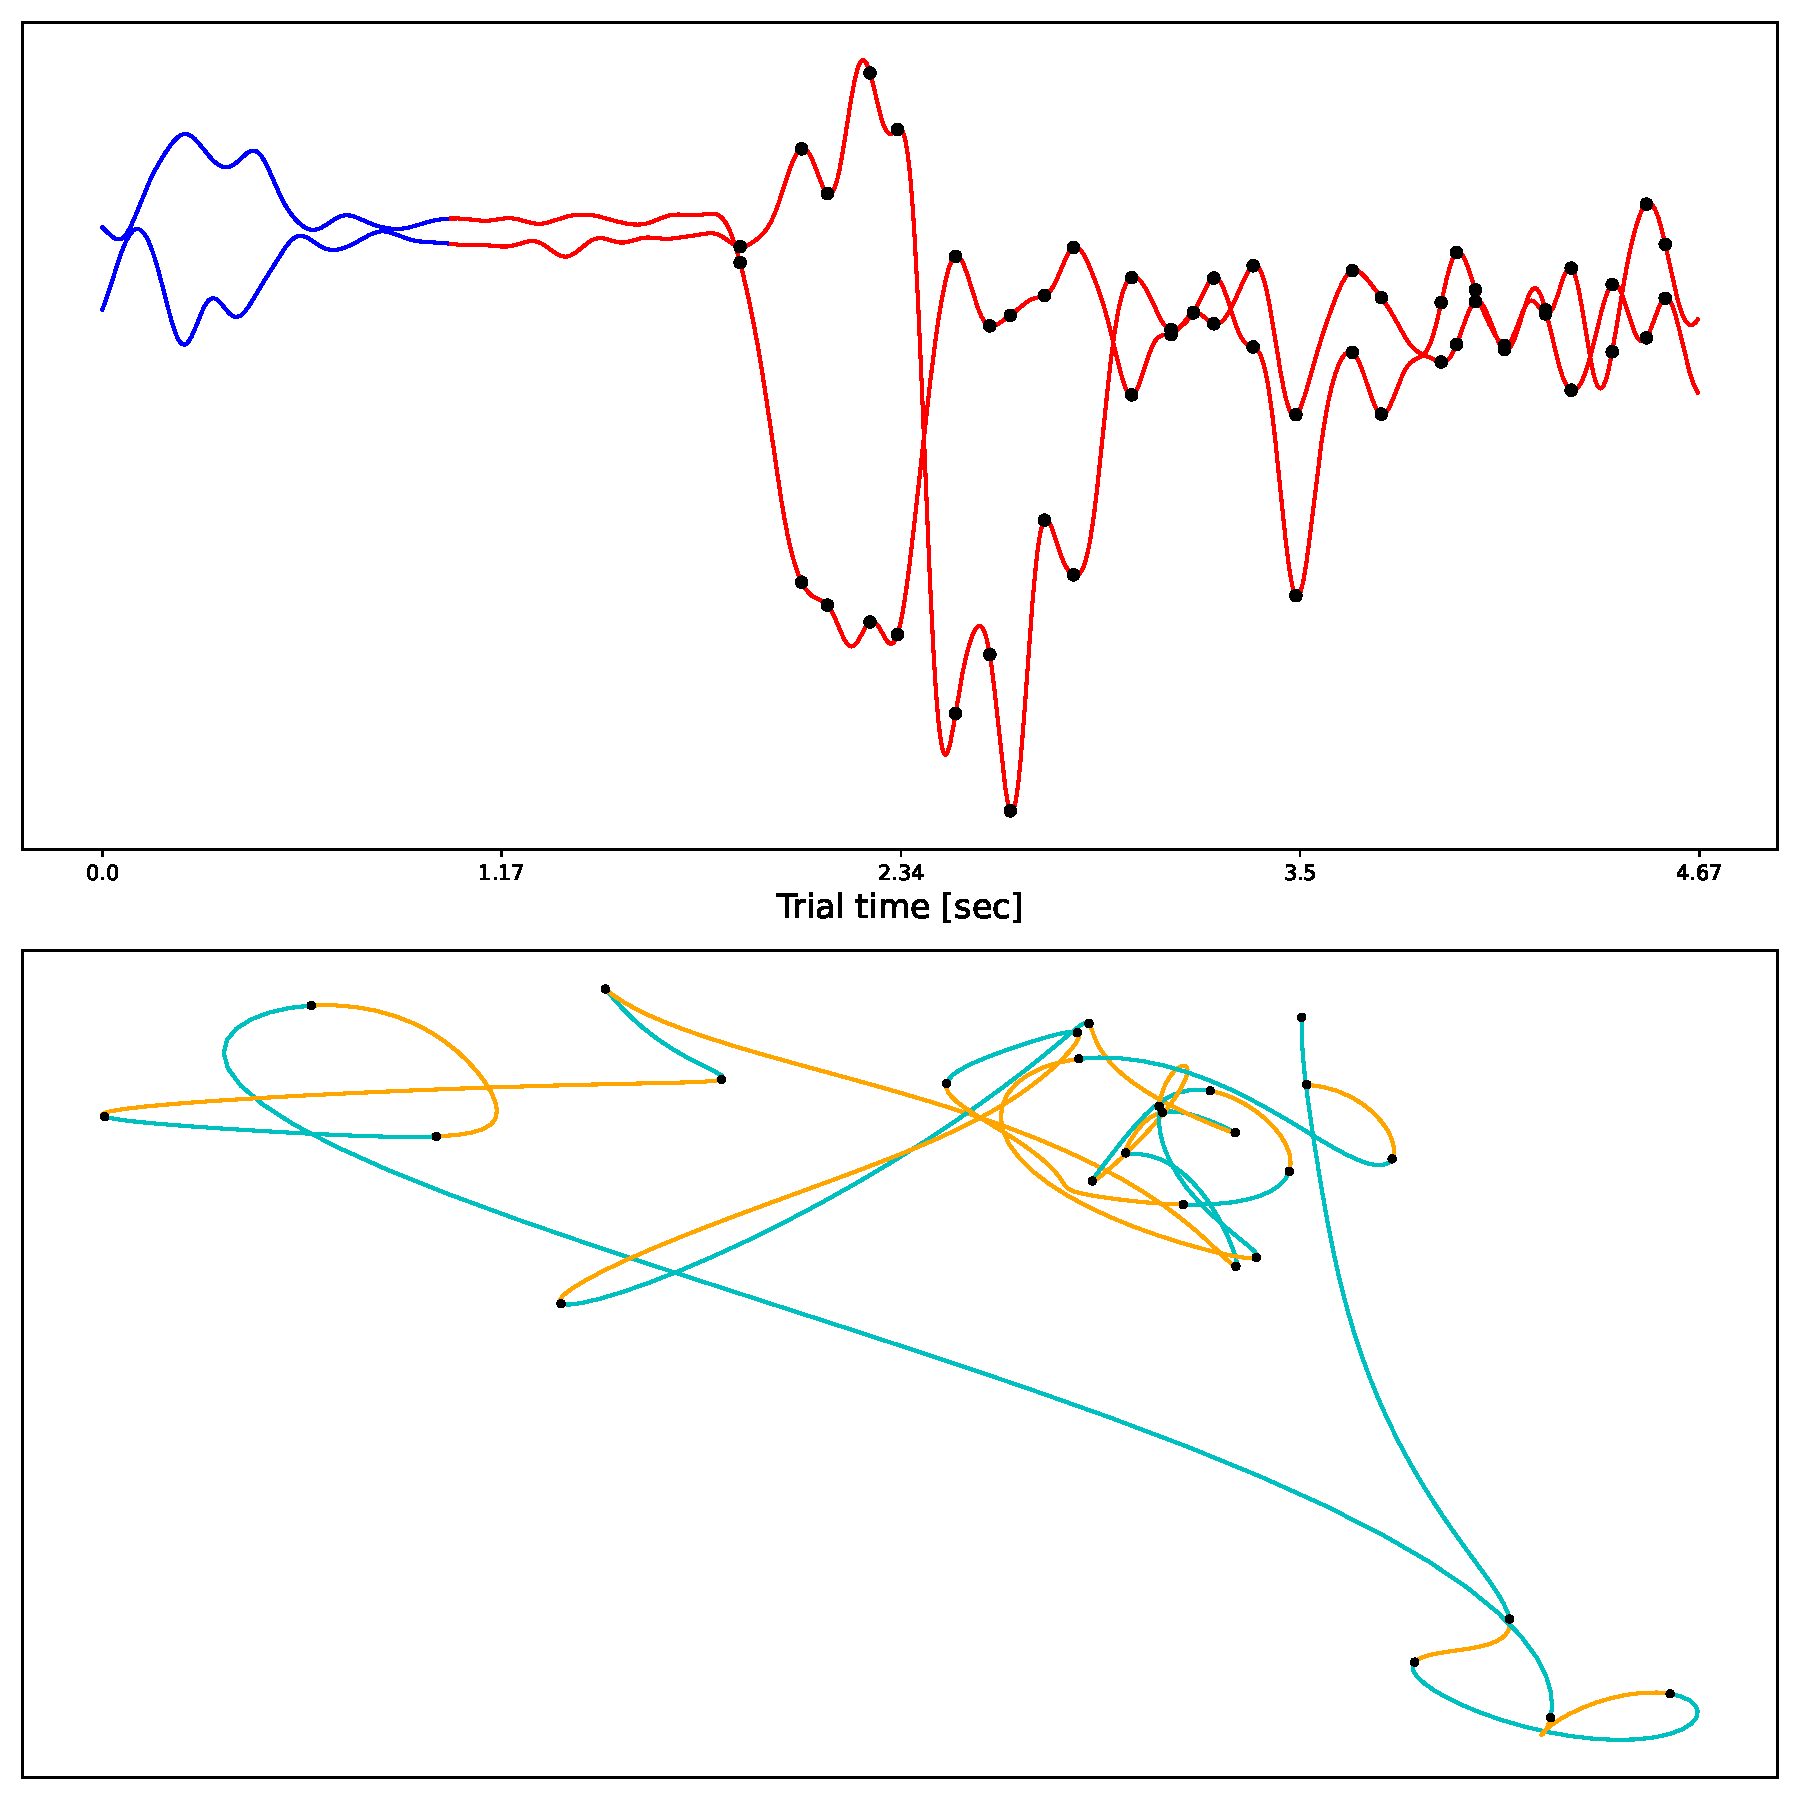
\includegraphics[width=1.0\textwidth]{basic_results/performance_over_blocks/example_path_segments.pdf}
    \caption[Trajectory segment definition]{zero crossings are diff (sign (diff (x))), then filter crossings that are within a time interval and above a minimum velocity as a percentage of the max}\label{fig:segments}
\end{figure}


Reward is defined over $K$ trials and samples or timepoints $T$ as:

\begin{align}
    r = \frac{1}{KT}\sum_k^K\sum_t^T{|| \vec{g_k} - \vec{x}_{t,k} ||^2}.
    \label{eq:reward}
\end{align}

\begin{figure}[tph]
    \centering
    \includegraphics[width=0.8\textwidth]{basic_results/performance_over_blocks/hit_fraction_vs_reward.pdf}
    \caption[Hits versus reward]{Fractions of trial outcome types for each block of the center-hold, reach-out task. Hit fraction increases on each trial, suggesting the beginnings of task learning. Hold timeout failure increases over trials as well, perhaps suggesting increased baseline excitation of muscles during the hold period. Part of learning to activate certain muscle modes is learning to inhibit others.}\label{fig:hit_fraction_vs_reward}
\end{figure}


\cref{eq:reward}


\begin{figure}[tph]
    \centering
    \includegraphics[width=1.0\textwidth]{basic_results/performance_over_blocks/mean_rewards_vs_learning_rate.pdf}
    \caption[Reward versus learning rate]{No correlation!}\label{fig:mean_rewards_vs_learning_rate}
\end{figure}


\begin{table}[H]
    \begin{center}
        \caption[Statistics of performance regression]{Statistics of performance regression}\label{tab:performance_stats}
        \begin{tabular}{l | c}
            \hline
            $p$(Hit Learning Rate, Reward) & 0.177 \\
            $p$(Reach time Learning Rate, Reward) & 0.215 \\
            $p$(Path length Learning Rate, Reward) & 0.786 \\
            $p$(Segment Learning Rate, Reward) & 0.072 \\
            Adjusted R-squared & 0.058 \\
            Prob (F-statistic) & 0.170
        \end{tabular}
    \end{center}
  \end{table}
  
% mean_reward vs [hit_learning_rates, reach_time_learning_rates, path_length_learning_rates, segment_learning_rates]

% OLS Regression Results                            
% ==============================================================================
% Dep. Variable:                      y   R-squared:                       0.142
% Model:                            OLS   Adj. R-squared:                  0.058
% Method:                 Least Squares   F-statistic:                     1.693
% Date:                Wed, 14 Feb 2024   Prob (F-statistic):              0.170
% Time:                        10:31:57   Log-Likelihood:               -0.99915
% No. Observations:                  46   AIC:                             12.00
% Df Residuals:                      41   BIC:                             21.04
% Df Model:                           4                                         
% Covariance Type:            nonrobust                                         
% ==============================================================================
%                  coef    std err          t      P>|t|      [0.025      0.975]
% ------------------------------------------------------------------------------
% const          0.9233      0.114      8.083      0.000       0.693       1.054
% x1             0.0780      0.057      1.375      0.177      -0.037       0.193
% x2             0.7350      0.584      1.259      0.215      -0.444       1.914
% x3             0.0102      0.037      0.274      0.786      -0.065       0.085
% x4            -0.1088      0.059     -1.845      0.072      -0.228       0.010
% ==============================================================================
% Omnibus:                        4.990   Durbin-Watson:                   2.155
% Prob(Omnibus):                  0.083   Jarque-Bera (JB):                4.054
% Skew:                           0.477   Prob(JB):                        0.132
% Kurtosis:                       4.098   Cond. No.                         51.4
% ==============================================================================



\begin{figure}
    \centering
    \begin{minipage}{0.49\textwidth}
        \includegraphics[width=0.9\textwidth]{basic_results/trial_reward/reward_histogram.pdf}
        \subcaption{}
    \end{minipage}
    \begin{minipage}{0.49\textwidth}
        \includegraphics[width=0.9\textwidth]{basic_results/trial_reward/hit_fraction_histogram.pdf}
      \subcaption{}
    \end{minipage}
    \caption[Hit and reward histograms]{Hits and rewards histograms over subjects}\label{fig:reward_histograms}
\end{figure}



\subsection{Hits over Targets}

\begin{figure}[tph]
    \centering
    \begin{minipage}{0.49\textwidth}
        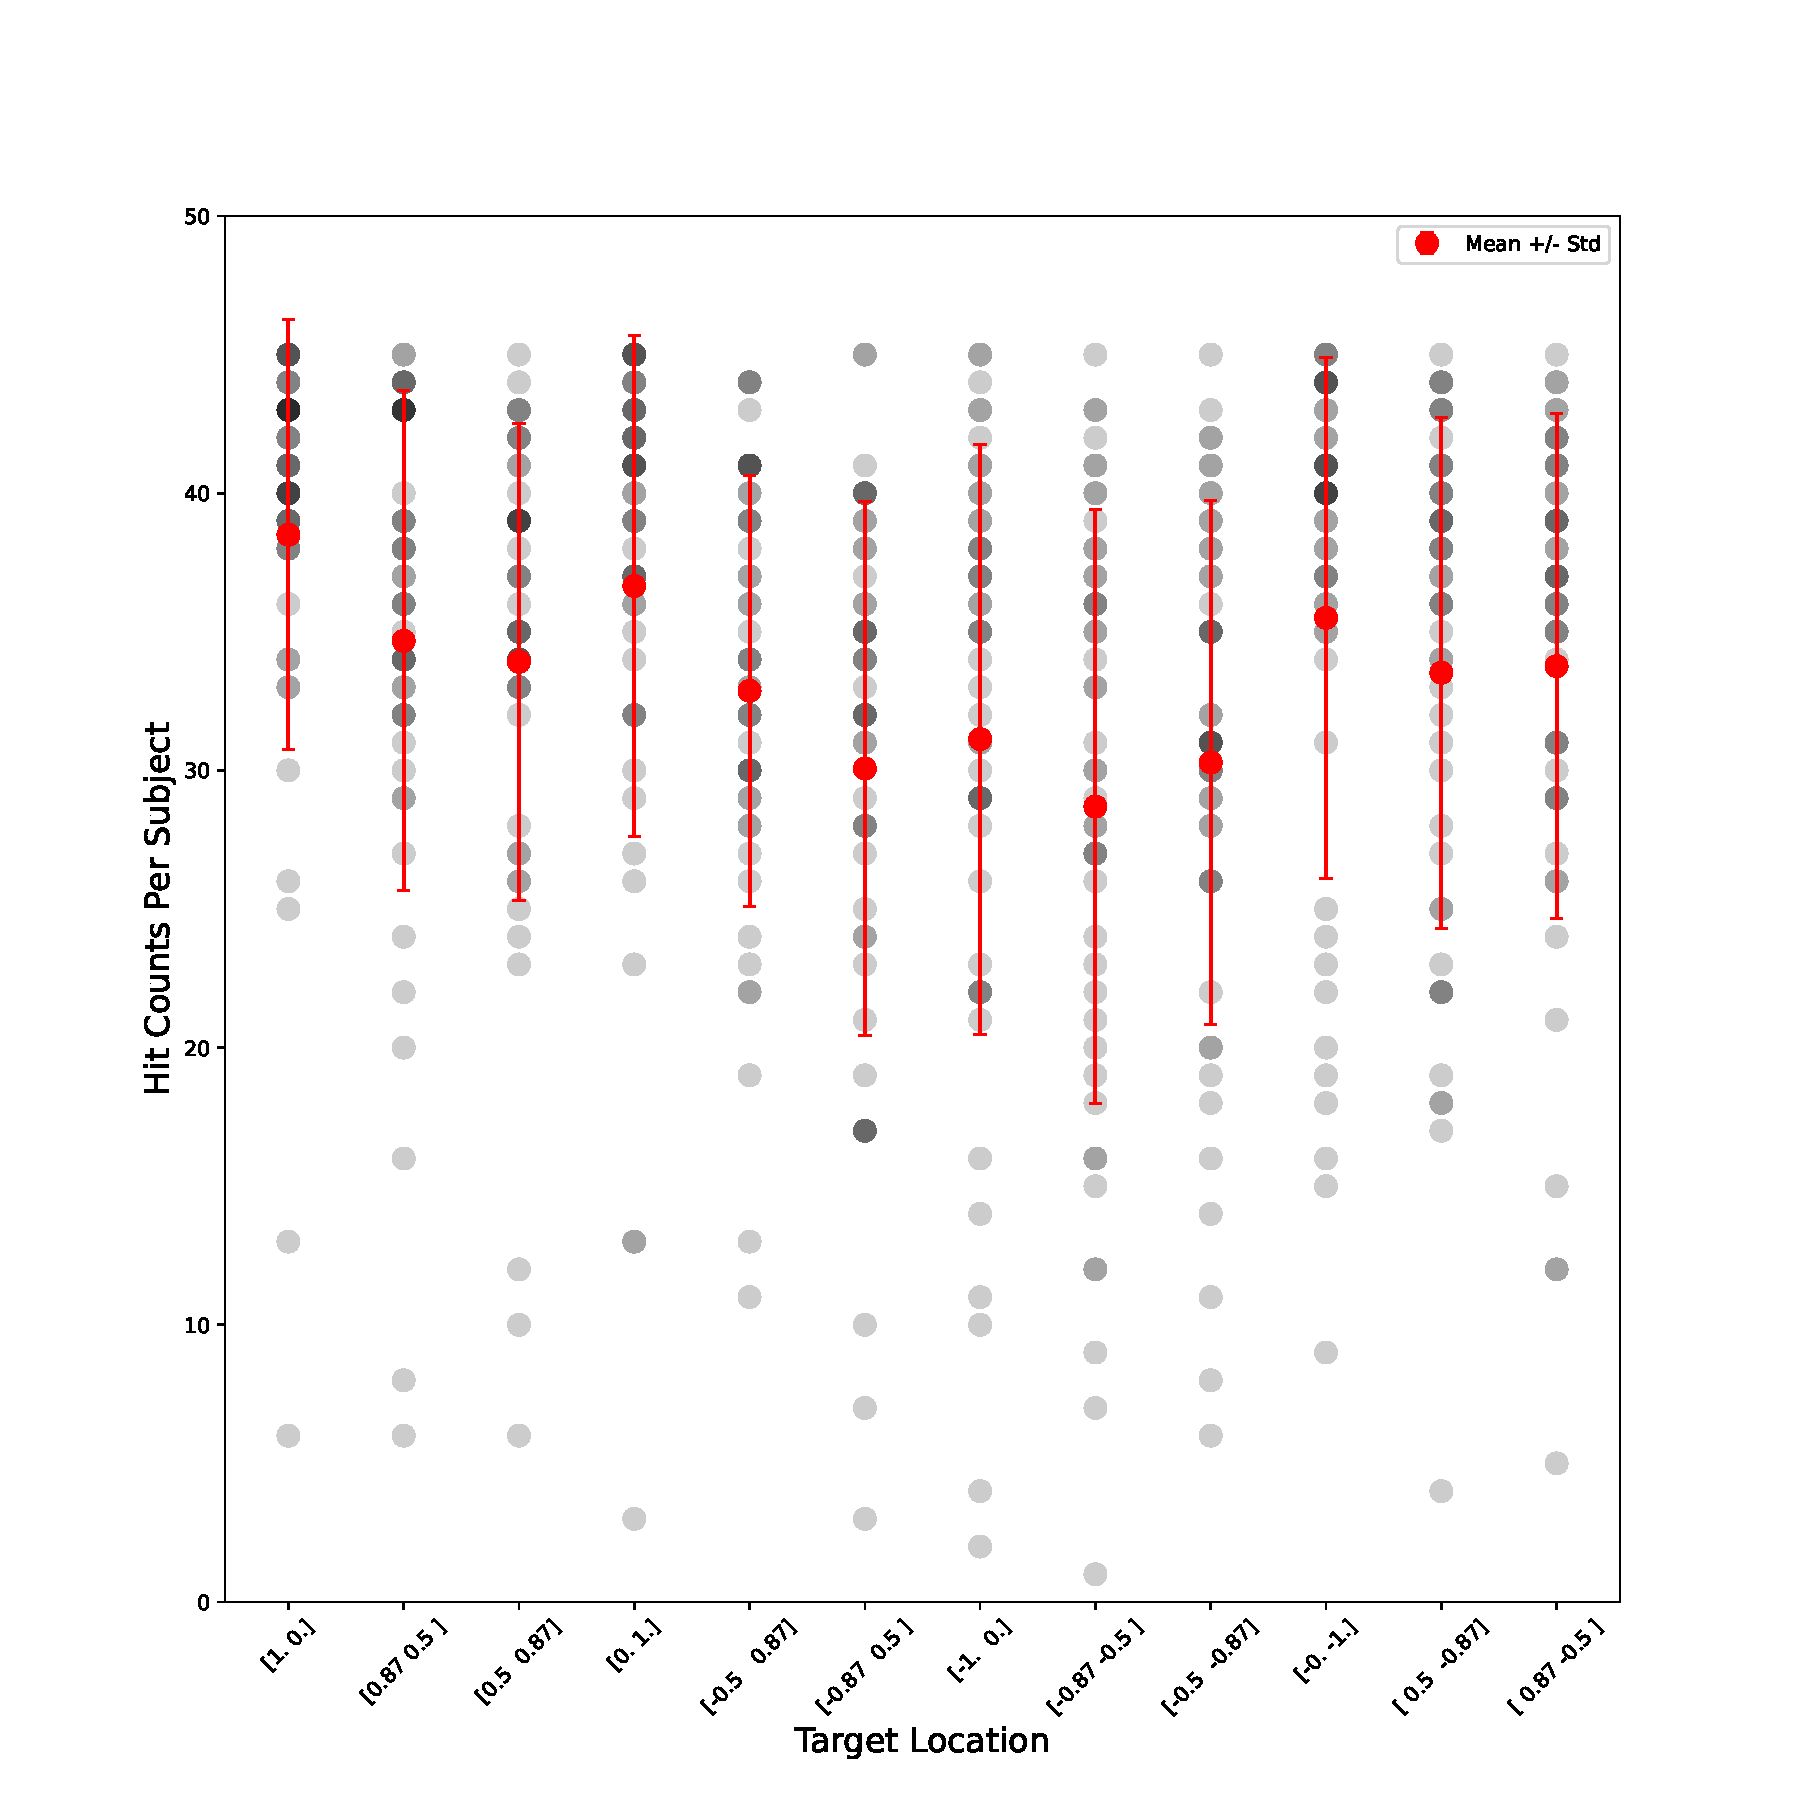
\includegraphics[width=0.95\textwidth]{basic_results/decoder_vs_performance/hits_over_targets.pdf}
        \subcaption{}
    \end{minipage}
    \begin{minipage}{0.49\textwidth}
        \includegraphics[width=0.85\textwidth]{basic_results/decoder_vs_performance/target_means.pdf}
      \subcaption{}
    \end{minipage}
    \caption[Hits over targets]{Hits over targets}\label{fig:hits_over_targets}
\end{figure}


\begin{figure}[tph]
    \centering
    \includegraphics[width=0.8\textwidth]{basic_results/decoder_vs_performance/target_hit_pvalues.pdf}
    \caption[Target hit Tukey test]{??}\label{fig:target_hit_pvalues}
\end{figure}

\Cref{fig:target_hit_pvalues}
\Cref{fig:target_hit_pvalues}


% Table showing p-values for target subject mean hit fraction differences:
% 
% \begin{table}[H]
% \begin{center}
%     \caption{}\label{table:}
%     \begin{tabular}{ c | c }
%         Target Pair & $p$-value \\
%         \hline
%         1, 6  & 1.085e-03 \\ 
%         1, 7  & 9.567e-03 \\ 
%         1, 8  & 4.629e-05 \\ 
%         1, 9  & 1.830e-03 \\ 
%         4, 6  & 4.040e-02 \\ 
%         4, 8  & 3.251e-03 \\ 
%         8, 10  & 2.783e-02 \\ 
%     \end{tabular}
% \end{center}
% \end{table}



\section{Do Subject Attributes Predict Performance?}

Look at self-reported form response data (this should show that there aren’t obvious confounds, as far as we can tell?)
    Arm size
    Time of day
    Time order
    Max “force” – sum of the channel variances?
    Caffeine vs. non
    Instrument players vs. non

\begin{figure}[tph]
    \centering
    \includegraphics[width=1.0\textwidth]{basic_results/form_response/arm_vs_reward.pdf}
    \caption[Arm versus reward]{}\label{fig:arm_vs_reward}
\end{figure}

\begin{figure}[tph]
    \centering
    \includegraphics[width=1.0\textwidth]{basic_results/form_response/days_vs_reward.pdf}
    \caption[Experiment day versus reward]{}\label{fig:days_vs_reward}
\end{figure}

\begin{figure}[tph]
    \centering
    \includegraphics[width=1.0\textwidth]{basic_results/form_response/hour_of_day_vs_reward.pdf}
    \caption[Hour of day versus reward]{}\label{fig:hour_of_day_vs_reward}
\end{figure}

\begin{figure}[tph]
    \centering
    \includegraphics[width=1.0\textwidth]{basic_results/form_response/sleep_vs_reward.pdf}
    \caption[Hours of sleep vs reward]{}\label{fig:sleep_vs_reward}
\end{figure}

\begin{figure}[tph]
    \centering
    \includegraphics[width=1.0\textwidth]{basic_results/form_response/compare_subject_groups.pdf}
    \caption[Subject group comparisons]{}\label{fig:compare_subject_groups}
\end{figure}



\section{Does the Decoder Predict Performance?}

Digging into the decoder

Do the directions of the decoder correlate with performance? 
    Hypothesis: yes, decoder directions which happen to be oriented towards targets will make the learning problem easier, and thus correlate positively with performance.

If the decoder directions are more/less aligned to the target directions, do subjects explore less/more? Is exploration (e.g. EMG variance) higher in subjects with misaligned decoders?
    Hypothesis: exploration will be lower in subjects with target-aligned decoders. Subjects make fewer incorrect movements, and thus are induced to explore less.

\begin{figure}[tph]
    \centering
    \includegraphics[width=1.0\textwidth]{basic_results/decoder_vs_performance/decoder_arrows.pdf}
    \caption[Example decoder directions in 2D.]{Example decoders directions in 2D.}\label{fig:decoder_arrows}
\end{figure}

\begin{figure}[tph]
    \centering
    \includegraphics[width=1.0\textwidth]{basic_results/decoder_vs_performance/decoder_normality_test.pdf}
    \caption[Decoder normality testing]{Testing the effect of the decoder on uniform data.}\label{fig:decoder_normality}
\end{figure}

\begin{figure}[tph]
    \centering
    \includegraphics[width=1.0\textwidth]{basic_results/decoder_vs_performance/decoder_cosine_vs_reward.pdf}
    \caption[Decoder axis similarity versus reward]{Decoder cosine similarity. EMG-to-force decoders are computed using a calibration dataset collected before the ``center hold, reach out'' task. 4 ``modes'' of EMG activity are extracted from the dataset using non-negative matrix factorization. These 4 modes are then subtracted in pairs to yield the two 64-dimensional EMG-to-force mappings, shown in \{+@fig:low\_variance\_PCs\}. The left plot shows the cosine similarity of the $x$ and $y$ EMG-to-force decoders. A cosine similarity of 1 means the two vectors are parallel, producing identical forces (in the respective directions) for the same EMG activity ($F_x = F_y$). A cosine similarity of -1 means the vectors are antiparallel, producing equal but opposite forces in the two directions ($F_x = -F_y$). A cosine similarity of 0 means the decoder directions are orthogonal; e.g.~producing a force in the $x$ direction with a certain EMG activity produces no force in the $y$ direction. Plotted across subjects, we see a range of decoder similarities, providing a variety of task contingencies. The rightmost plot asks whether cosine similarity is predictive of task success, in terms of the numbers of ``Hits''. We find no significant correlation, implying that the decoder cosine similarity, in the range we tested, does not predict task success. Task success, therefore, likely relies on an alternative task variable.}\label{fig:decoder_cosine_vs_reward}
\end{figure}



\section{Does Task Space Variance Decrease over Trials?}

Trajectory viz, discussion, stats (task space only)
Look at histograms over trials for x and y – where are people moving over time?
Look at trajectory means, trajectory distros
Show 2D histograms, mean trajectories
What must be happening in the EMG space to get these trajectories?
This is all “on manifold”-- what’s happening off-manifold?
Histos to show if any subjects are outliers that we should ignore
Who are the “best” subjects in terms of trajectories? Note these as a subgroup that we can zoom in on later.


\begin{figure}[tph]
    \centering
    \includegraphics[height=0.9\textheight]{basic_results/mean_trajectories/mean_trajectories.pdf}
    \caption[Mean trajectories]{??}\label{fig:mean_trajectories}
\end{figure}


\begin{figure}[tph]
    \centering
    \includegraphics[width=\textwidth]{basic_results/trajectory_variance/rotated_trajectories.pdf}
    \caption[Rotating trajectories]{??}\label{fig:rotated_trajectories}
\end{figure}


\begin{figure}[tph]
    \centering
    \includegraphics[width=0.9\textwidth]{basic_results/trajectory_variance/trajectory_variance_over_blocks.pdf}
    \caption[Trajectory variance over blocks]{Plotting the log as variance tends to decrease exponentially}\label{fig:trajectory_variance}
\end{figure}


\begin{figure}[tph]
    \centering
    \begin{minipage}{0.9\textwidth}
        \includegraphics[width=\textwidth]{basic_results/trajectory_variance/trajectory_r_squared_fit.pdf}
        \subcaption{}
    \end{minipage}\\%
    \begin{minipage}{0.9\textwidth}
        \includegraphics[width=0.8\textwidth]{basic_results/trajectory_variance/trajectory_variance_slope.pdf}
      \subcaption{}
    \end{minipage}
    \caption[Trajectory variance statistics]{Trajectory variance statistics}\label{fig:trajectory_variance_fits}
\end{figure}




\cleardoublepage\printendnotes%
\ifSubfilesClassLoaded{%
    \newpage%
    \bibliography{../bib/bibliography}%
}{}%
\end{document}